\section{The horizon lesson}

\begin{figure}[t]
\centering
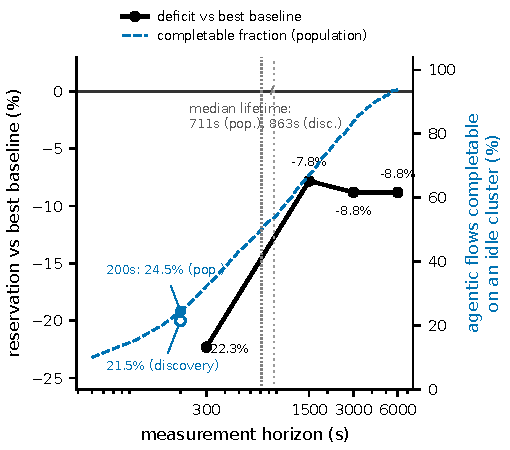
\includegraphics[width=3.4in]{figures/F4_horizon_lesson.pdf}
\caption{Horizon censoring on one core cell. The population median agentic flow lifetime, derived from the released workload generators, is roughly 711 seconds (first measured at 863 seconds on the diagnostic realization that surfaced the artifact, open markers); at a 200-second window only about a quarter of agentic flows can complete even on an idle cluster (24.5 percent of the population; 21.5 percent of the diagnostic realization), while the campaign's default horizons ran 150 to 300 seconds. The measured deficit is 22.3 percent at a 300-second horizon and halves to 7.8 percent at adequate horizons, stable through 6000 seconds. Horizons shorter than the workload's completable lifetimes charge guarantee-holders full stranding cost against zero completion payoff (Section 8).}
\label{fig:f4}
\end{figure}

The evaluation's most generalizable finding is about measurement, and it
was found the way such things are found: by investigating a suspicious
zero. The starvation diagnostic of Section 7.4 revealed, alongside the
genuine starvation, that every sweep in the campaign was running a
measurement horizon far shorter than the workload's own timescale. The
median agentic flow requires roughly 711 seconds to complete with no
queueing at all, tool-time gaps plus decode service; the figure was
first measured at roughly 863 seconds on the diagnostic realization
that surfaced the problem, and the released generator derivation, which
any reader can run, gives 711. The build's default horizons ran 150 to
300 seconds, and at a 200-second window only about a quarter of agentic
flows (24.5 percent of the population; 21.5 percent of the diagnostic
realization) could complete on an idle cluster. The primary metric counts completed
flows. A window shorter than the unit of value does not measure the
metric; it measures truncation.

The bias is not symmetric, and it points at completion-guaranteeing
policies specifically. A reservation pays its stranding cost during the
flow and collects its payoff at completion; a horizon that ends before
completion charges the full cost against zero payoff, the mechanism's
worst case by construction, while policies that never schedule long flows
at all are barely touched. Quantified on one core cell (Figure 4), the
discipline's deficit against the best baseline was 22.3 percent at a
300-second horizon and 7.8 percent at 1500 seconds, stable through 6000
seconds; at the longest horizon the discipline completed more flows in
absolute terms than its comparator while still losing on value-weighted
goodput, a real loss, but half the reported one.

The subtler effect is that censoring corrupts tuning, not only
measurement. Re-tuning every policy at the corrected horizon flipped
selected parameters across the board, most cleanly for the multi-level
feedback baseline, whose chosen quantum moved from the shortest value in
its grid to the longest, in every workload family. Under a censored
horizon, aggressive demotion looks good because long flows are truncated
before their cost lands; correct the horizon and the same tuner, on the
same grid, chooses patience. An evaluation that had tuned at 300 seconds
and measured at 1500 would have compared the mechanism against baselines
mis-tuned in its favor. Both tuning campaigns are released.

The fix is structural, not vigilant: the released code asserts, before any
sweep runs, that the configured horizon exceeds the workload's derivable
median flow lifetime, and the verdict path independently rejects any
manifest whose horizon disagrees with the grid it claims to report. The
correction was adopted as a numbered amendment before the final grid ran,
under a one-fix clause barring further measurement changes in either
direction, and its full history, including that the correction improved
the mechanism's number on the probe cell and worsened it on H2, is in the
released amendment log. The rule generalizes to any completion-metric
evaluation of long-horizon agents, a category currently multiplying:
horizons must exceed the completable-lifetime distribution of the workload,
or the benchmark measures its own window. We found the cost of honoring
this rule to be severe, superlinear in the horizon under sustained
overload, and it forced a disclosed reduction of our own grid; we suspect
the rule is widely violated for exactly this reason.
